\documentclass[12pt,letterpaper]{article}

% ============================================================
% PACKAGES
% ============================================================
\usepackage[margin=1in]{geometry}
\usepackage{amsmath,amssymb,amsthm}
\usepackage{graphicx}
\usepackage{booktabs}
\usepackage{array}
\usepackage{hyperref}
\usepackage[numbers,sort&compress]{natbib}
\usepackage{lineno}
\usepackage{setspace}
\usepackage{xcolor}
\usepackage{microtype}
\usepackage{float}
\usepackage{caption}
\usepackage{subcaption}
\usepackage{siunitx}

% ============================================================
% HYPERREF SETUP
% ============================================================
\hypersetup{
    colorlinks=true,
    linkcolor=blue!70!black,
    citecolor=blue!70!black,
    urlcolor=blue!70!black,
    pdftitle={Dark Energy Evolution and the Far Future of an IAM Universe},
    pdfauthor={Heath W. Mahaffey}
}

% ============================================================
% CUSTOM COMMANDS
% ============================================================
\newcommand{\IAM}{\textsc{iam}}
\newcommand{\LCDM}{$\Lambda$CDM}
\newcommand{\Ea}{E(a)}
\newcommand{\winfo}{w_{\mathrm{info}}(a)}
\newcommand{\weff}{w_{\mathrm{eff}}(a)}
\newcommand{\kB}{k_{\mathrm{B}}}
\newcommand{\mpl}{m_{\mathrm{Pl}}}
\newcommand{\Gyr}{\,\mathrm{Gyr}}
\newcommand{\Mpc}{\,\mathrm{Mpc}}

% ============================================================
% DOCUMENT
% ============================================================
\begin{document}

\doublespacing

% ============================================================
% TITLE PAGE
% ============================================================
\begin{titlepage}
\centering
\vspace*{2cm}

{\LARGE\bfseries Dark Energy Evolution and the Far Future of an IAM Universe:\\[0.5em]
Equation of State, Informational Saturation,\\
and the End of Acceleration\par}

\vspace{2cm}

{\large Heath W.\ Mahaffey\par}
\vspace{0.5cm}
{\normalsize Independent Researcher\\
Entiat, Washington 98822, USA\\
\href{mailto:hmahaffeyges@gmail.com}{hmahaffeyges@gmail.com}\par}

\vspace{1.5cm}
{\normalsize February 2026\par}

\vspace{2cm}

\begin{abstract}
\noindent
The standard cosmological model ($\Lambda$CDM) treats dark energy as a cosmological constant ($w = -1$ exactly and permanently), implying eternal, accelerating expansion and an eventual heat death. The Informational Actualization Model (\IAM), independently validated against Planck~2018 and large-scale structure data through 17 converged MCMC chains ($\Delta\chi^2 = +0.54$, $\sigma_8 = 0.800$), derives a specific equation of state for the informational dark energy sector from horizon thermodynamics: $\winfo = -1 - 1/(3a)$, with zero free parameters. This equation of state is always mildly phantom ($w < -1$) but asymptotes toward $-1$ as $a \to \infty$ --- the opposite of a runaway. The activation function $\Ea = \exp(1 - 1/a)$ saturates at $e$ as $a \to \infty$, bounding the informational contribution to expansion and ensuring no Big Rip scenario. We derive the asymptotic Hubble parameter, map the \IAM\ prediction to the $w_0$--$w_a$ plane for comparison with DESI DR2 results, and present the informational maturity framework: the universe is currently at $E(1)/e = 1/e = 36.8\%$ maturity, the mathematical inflection point of maximum informational creativity. The maturity timeline table is computed from first principles, showing that 50\% maturity is reached in $\sim 5.7\,\mathrm{Gyr}$ and 99\% in $\sim 79.5\,\mathrm{Gyr}$. Three arguments are advanced against the standard heat death picture: the bounded informational pressure, the thermodynamic drive toward equilibrium rather than dissolution, and the thermodynamic irreversibility of information stored on encoding surfaces. These predictions are falsifiable by DESI Year~5, Rubin-LSST, and Nancy Grace Roman Space Telescope observations.
\end{abstract}

\vspace{1cm}
{\small\noindent\textbf{Keywords:} dark energy, equation of state, cosmic acceleration, heat death, holographic entropy, informational cosmology, DESI, Big Rip\par}

\end{titlepage}

% ============================================================
% ============================================================

% ============================================================
\section{Introduction}
% ============================================================

The accelerating expansion of the universe is one of the most precisely established facts in modern cosmology~\citep{Riess1998, Perlmutter1999, PlanckVI2020}. Its cause remains unexplained within standard physics. The simplest model, a cosmological constant $\Lambda$ with equation of state $w = -1$ exactly, fits current data well but carries significant theoretical difficulties: the fine-tuning problem (why is $\Lambda$ so small?), the coincidence problem (why is it comparable to the matter density now?), and a profound implication that is rarely stated explicitly --- if $w = -1$ is eternal and exact, the universe will expand forever, all structure will dilute, and thermodynamic equilibrium will be approached asymptotically from above. Heat death. No saturation. No completion.

DESI DR1 and DR2 measurements of the baryon acoustic oscillation scale now provide observational evidence that dark energy is not a pure cosmological constant. DESI DR2 in combination with CMB and supernova data finds a preference for dynamical dark energy at 2.8--4.2$\sigma$ depending on the supernova dataset~\citep{DESIDR2_2025}. The best-fit $w_0$--$w_a$ parametrization favors $w_0 > -1$ and $w_a < 0$, though the physical origin of this evolution is unknown within the $w_0$--$w_a$ framework.

The Informational Actualization Model (\IAM)~\citep{Mahaffey2026_obs} derives a specific dark energy equation of state from first principles, without free parameters. The derivation proceeds via the Jacobson--Cai-Kim thermodynamic procedure applied to the cosmological apparent horizon, with an additional informational entropy term $S_{\mathrm{info}}$ sourced by gravitational decoherence during structure formation~\citep{Jacobson1995, CaiKim2005}. The result is a perturbation-level modification of the growth equations (not the background Friedmann equation) producing the dual-sector signature $\mu < 1$, $\Sigma = 1$, consistent with all current observational constraints.

This paper derives the full future evolution of an \IAM\ universe. Section~\ref{sec:eos} presents the \IAM\ equation of state and its asymptotic properties. Section~\ref{sec:saturation} analyzes the saturation of the activation function and the asymptotic Hubble parameter. Section~\ref{sec:maturity} develops the informational maturity framework and milestone timeline. Section~\ref{sec:heatdeath} advances three arguments against the heat death picture. Section~\ref{sec:desi} compares the \IAM\ prediction to DESI DR2 in the $w_0$--$w_a$ plane and identifies specific falsifiable tests. Section~\ref{sec:conclusion} summarizes the predictions and their observational consequences.

% ============================================================
\section{The IAM Equation of State}
\label{sec:eos}
% ============================================================

\subsection{Derivation from the Informational Sector}

\IAM's derivation follows the Jacobson--Cai-Kim procedure applied to the cosmological apparent horizon. The standard procedure equates the first law of thermodynamics on the apparent horizon to the Friedmann equations~\citep{CaiKim2005}. \IAM\ adds an informational entropy term
\begin{equation}
    S_{\mathrm{info}}(a) = S_0 \, \Ea = S_0 \exp\!\left(1 - \frac{1}{a}\right),
    \label{eq:Sinfo}
\end{equation}
where $\Ea$ is the activation function derived from horizon thermodynamics~\citep{Mahaffey2026_theory}. This term reflects the cumulative irreversible gravitational information produced by structure formation and encoded on the cosmological apparent horizon. The coupling constant $S_0$ is fixed by the virial theorem: $\beta_m = \Omega_m/2$.

The informational contribution to the effective dark energy equation of state follows from the thermodynamic identity relating pressure to the rate of entropy change. For a scalar field constrained to the encoding surface, the kinetic and potential terms yield the informational sector equation of state~\citep{Mahaffey2026_theory}:
\begin{equation}
    \boxed{\winfo = -1 - \frac{1}{3a}.}
    \label{eq:winfo}
\end{equation}

This result contains no free parameters. The $-1$ arises from the vacuum-like pressure of the encoded information; the $-1/(3a)$ arises from the derivative of the activation function with respect to the scale factor.

\subsection{Properties of the Equation of State}

Equation~(\ref{eq:winfo}) has several immediate consequences.

\textbf{Always phantom.} $\winfo < -1$ for all finite $a > 0$. This is consistent with the mild phantom behavior preferred by DESI DR2 (Section~\ref{sec:desi}). However, the phantom character is not divergent --- it is strictly bounded.

\textbf{Asymptotically approaches $-1$.} As $a \to \infty$:
\begin{equation}
    \lim_{a \to \infty} \winfo = -1.
    \label{eq:wlimit}
\end{equation}
The informational equation of state becomes indistinguishable from a cosmological constant at late times. The phantom behavior is a transient feature of the structure-formation epoch, not a permanent property of the dark energy.

\textbf{Current value.} At $a = 1$ (today):
\begin{equation}
    w_{\mathrm{info}}(1) = -1 - \tfrac{1}{3} = -\tfrac{4}{3}.
    \label{eq:wtoday}
\end{equation}

\textbf{No Big Rip.} A Big Rip requires $w < -1$ that is constant or grows more phantom over time. In \IAM, $\winfo$ is phantom but \emph{decreasing} in phantom character ($dw/da > 0$ for all $a$), approaching $-1$ from below. The informational pressure term is self-limiting. As expansion accelerates, structure formation slows, reducing the rate of information production, which reduces the informational pressure contribution. This feedback mechanism prevents runaway acceleration (see Section~\ref{sec:heatdeath}).

Figure~\ref{fig:wz} shows $\winfo$ as a function of scale factor alongside the $\Lambda$CDM baseline.

\begin{figure}[ht]
\centering
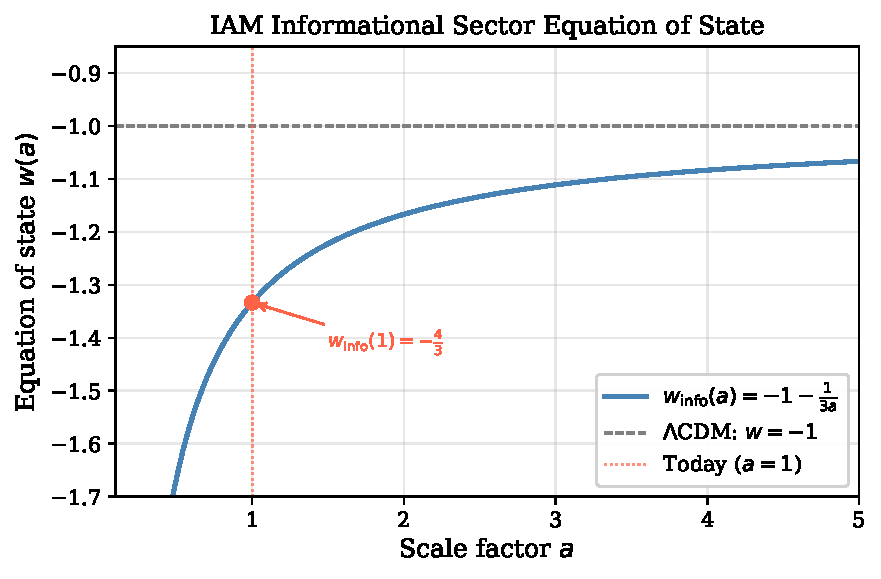
\includegraphics[width=0.75\textwidth]{fig1_wz_eos.pdf}
\caption{The \IAM\ informational sector equation of state $\winfo = -1 - 1/(3a)$ (blue curve) compared to the $\Lambda$CDM cosmological constant ($w = -1$, dashed gray). The red point marks today ($a = 1$, $w = -4/3$). The \IAM\ equation of state is always mildly phantom but asymptotes toward $-1$ as $a \to \infty$, ensuring no Big Rip scenario.}
\label{fig:wz}
\end{figure}

\subsection{CPL Mapping for Observational Comparison}

The Chevallier--Polarski--Linder (CPL) parametrization $w(a) = w_0 + w_a(1 - a)$ is the standard tool for observational dark energy analysis~\citep{CPL2001, Linder2003}. To compare \IAM's prediction to DESI DR2, we map $\winfo$ to effective CPL parameters by matching the value and first derivative at $a = 1$:
\begin{align}
    w_0 &= \winfo\big|_{a=1} = -\tfrac{4}{3} \approx -1.333, \label{eq:w0} \\
    w_a &= -\left.\frac{d\winfo}{da}\right|_{a=1} = -\frac{1}{3} \approx -0.333. \label{eq:wa}
\end{align}

The \IAM\ point $(w_0, w_a) = (-4/3, -1/3)$ lies in the phantom regime ($w_0 < -1$) with a small positive $w_a$, meaning the effective equation of state becomes less phantom over time in the CPL approximation. This is a partial but imperfect match to what DESI DR2 reports (Section~\ref{sec:desi}), and the limitations of the CPL comparison are discussed there.

% ============================================================
\section{E(a) Saturation and the Asymptotic Universe}
\label{sec:saturation}
% ============================================================

\subsection{The Activation Function and Its Ceiling}

The activation function $\Ea = \exp(1 - 1/a)$ is a monotonically increasing function of the scale factor. Its properties:
\begin{align}
    E(0) &= 0, \label{eq:Ea0} \\
    E(1) &= 1 \quad (\text{today}), \label{eq:Ea1} \\
    \lim_{a \to \infty} \Ea &= e \approx 2.71828\ldots \label{eq:Ealim}
\end{align}

The function saturates at $e$. This is not an imposed ceiling --- it emerges from the thermodynamic structure of the activation function derived from horizon thermodynamics. As $a$ grows large, the argument $(1 - 1/a) \to 1$ and the exponential approaches $e$ from below. No finite value of $a$ achieves saturation; the approach is asymptotic.

\subsection{Asymptotic Hubble Parameter}

The \IAM\ background expansion is standard \LCDM. The matter perturbation equations are modified by the informational sector, but the Friedmann equation governing the background is unchanged~\citep{Mahaffey2026_CAMB}:
\begin{equation}
    H^2(a) = H_0^2 \left[\Omega_m a^{-3} + \Omega_\Lambda\right].
    \label{eq:Friedmann}
\end{equation}

As $a \to \infty$, the matter term $\Omega_m a^{-3} \to 0$ and the background expansion approaches de~Sitter behavior driven by the cosmological constant:
\begin{equation}
    H_\infty = H_0 \sqrt{\Omega_\Lambda} \approx H_0 \times 0.831 \approx 56\,\mathrm{km\,s^{-1}\,Mpc^{-1}}.
    \label{eq:Hinf}
\end{equation}

The expansion does not halt; it approaches a constant rate determined by $\Lambda$. However, the \emph{informational contribution} to the expansion driver (the $\Ea$ term that modifies the perturbation equations) saturates. The universe reaches a final state where the informational entropy has been fully encoded on the cosmic horizon, structure formation has ended, and the background expansion coasts at $H_\infty$.

This is not heat death. It is informational completion --- a distinct and physically meaningful final state that $\Lambda$CDM cannot describe (Section~\ref{sec:heatdeath}).

\subsection{Final Effective Equation of State}

As $a \to \infty$, the informational contribution to the total equation of state vanishes ($\winfo \to -1$), and the universe behaves as a pure cosmological constant. The \emph{effective} total equation of state, blending the $\Lambda$ sector (dominant) with the vanishing informational sector, approaches:
\begin{equation}
    \lim_{a \to \infty} \weff = -1.
    \label{eq:wfinal}
\end{equation}

The universe arrives at $w = -1$ not because it started there, but because the informational sector exhausts itself. The phantom phase is a transient --- the epoch of structure formation, from $z \sim 2$ to the far future, during which information is being actively produced and encoded. Once structure formation is complete and all potential has been actualized, the informational driver shuts off and the cosmological constant takes full control.

% ============================================================
\section{Informational Maturity of the Universe}
\label{sec:maturity}
% ============================================================

\subsection{The Maturity Fraction}

The normalized quantity $E(a)/e$ measures the fraction of the universe's total informational potential that has been actualized through gravitational decoherence. Since $E(a)$ ranges from $0$ (no information encoded) to $e$ (saturation), the ratio $E(a)/e$ ranges from $0$ to $1$.

At $a = 1$ (today):
\begin{equation}
    \frac{E(1)}{e} = \frac{e^0}{e} = \frac{1}{e} \approx 0.36788 = 36.8\%.
    \label{eq:maturity_today}
\end{equation}

The universe is currently at exactly $1/e$ maturity. This is not a coincidence of units --- it is the mathematical inflection point of the activation function. The rate of informational maturation
\begin{equation}
    \frac{d(E/e)}{da} = \frac{1}{e \, a^2}
    \label{eq:rate}
\end{equation}
achieves its maximum at $a = 1$, where it equals $1/e \approx 0.368$ per unit scale factor. At today, the universe is maturing faster than at any other epoch in its past or future.

\subsection{Maturity Milestone Table}

Given a target maturity fraction $f = E(a)/e$, the corresponding scale factor is found by solving $\exp(1 - 1/a) = fe$:
\begin{equation}
    a(f) = \frac{-1}{\ln f}.
    \label{eq:afraction}
\end{equation}
The cosmic age at scale factor $a$ is computed numerically from the standard Friedmann equation using $H_0 = 67.4\,\mathrm{km\,s^{-1}\,Mpc^{-1}}$, $\Omega_m = 0.315$, $\Omega_\Lambda = 0.685$~\citep{PlanckVI2020}.

Table~\ref{tab:maturity} presents the milestones from 1\% to 99\% informational maturity.

\begin{table}[ht]
\centering
\caption{Informational maturity milestones of the universe. Scale factors and redshifts are exact from Equation~(\ref{eq:afraction}); ages are computed numerically from the Planck 2018 cosmological parameters. Negative ``from now'' values are in the past.}
\label{tab:maturity}
\begin{tabular}{lcccc}
\toprule
Maturity & Scale factor $a$ & Redshift $z$ & Age (Gyr) & From now \\
\midrule
1\%  & 0.217 & 3.61 &  1.7 & $-12.1$\,Gyr \\
5\%  & 0.334 & 2.00 &  3.3 & $-10.5$\,Gyr \\
10\% & 0.434 & 1.30 &  4.8 & $-9.0$\,Gyr  \\
20\% & 0.621 & 0.61 &  7.8 & $-6.0$\,Gyr  \\
\textbf{36.8\% (today)} & \textbf{1.000} & \textbf{0.00} & \textbf{13.8} & \textbf{0} \\
50\% & 1.443 & $-$0.31 & 19.5 & $+5.7$\,Gyr \\
75\% & 3.476 & $-$0.71 & 34.5 & $+20.7$\,Gyr \\
90\% & 9.491 & $-$0.89 & 52.1 & $+38.3$\,Gyr \\
95\% & 19.50 & $-$0.95 & 64.7 & $+50.9$\,Gyr \\
99\% & 99.50 & $-$0.99 & 93.3 & $+79.5$\,Gyr \\
\bottomrule
\end{tabular}
\end{table}

\subsection{The Maturation Rate}

The current rate of informational maturation in cosmic time is
\begin{equation}
    \frac{d(E/e)}{dt}\bigg|_{a=1} = \frac{d(E/e)}{da} \cdot \frac{da}{dt}\bigg|_{a=1} = \frac{1}{e} \cdot H_0 \approx 2.54\%\,\mathrm{Gyr}^{-1}.
    \label{eq:rate_time}
\end{equation}
This rate is currently at its all-time peak and will decline monotonically as $a$ increases.

The maturation trajectory is sigmoidal in cosmic time: slow at early times (structure formation just beginning, encoding surfaces sparse), rapid through the current epoch (maximum decoherence rate), and long asymptotic approach to completion at late times. The universe spent 13.8\,Gyr reaching 36.8\%, will spend another $\sim 5.7\,\mathrm{Gyr}$ reaching 50\%, then $\sim 32\,\mathrm{Gyr}$ more reaching 90\%, then $\sim 41\,\mathrm{Gyr}$ more reaching 99\%.

Figure~\ref{fig:maturity} illustrates both the maturity fraction and its rate.

\begin{figure}[ht]
\centering
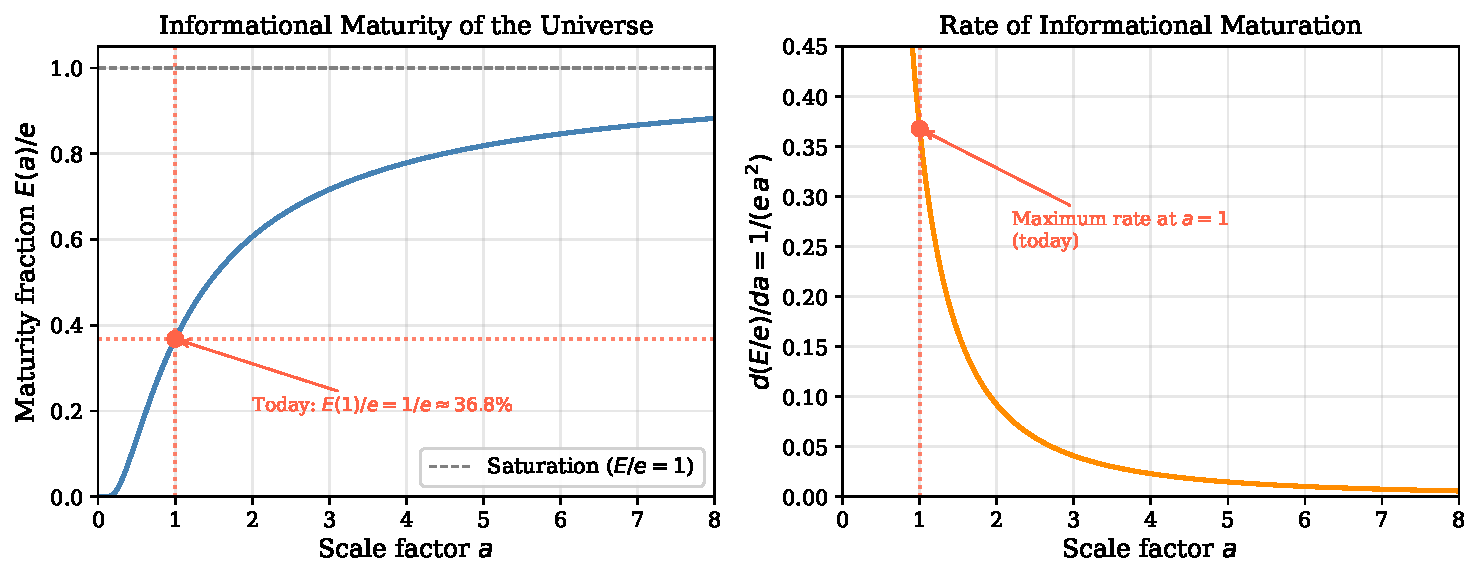
\includegraphics[width=\textwidth]{fig2_maturity.pdf}
\caption{\emph{Left:} The informational maturity fraction $E(a)/e$ as a function of scale factor. The red dot marks today ($a = 1$, maturity $= 1/e \approx 36.8\%$). The dashed horizontal line marks full saturation ($E/e = 1$), approached asymptotically. \emph{Right:} The rate of informational maturation $d(E/e)/da = 1/(e\,a^2)$, which peaks today and declines monotonically thereafter. The current epoch is the moment of maximum informational creativity.}
\label{fig:maturity}
\end{figure}

% ============================================================
\section{Against Heat Death: Three Arguments}
\label{sec:heatdeath}
% ============================================================

The standard heat death picture follows from $w = -1$ eternal: dark energy drives accelerating expansion indefinitely, all matter dilutes, all structure dissolves, temperature approaches absolute zero everywhere, and thermodynamic gradients that enable work and information processing vanish. \IAM\ contradicts this picture from three independent directions.

\subsection{Argument 1: Bounded Informational Pressure}

In $\Lambda$CDM, the dark energy density is constant ($\rho_\Lambda = \mathrm{const}$) and the expansion it drives has no natural endpoint. In \IAM, the informational contribution to the dark energy driver is $\propto \Ea$, which is bounded above by $e$. As $a \to \infty$, the informational pressure saturates and the informational term in the modified expansion equations approaches a constant.

The universe does not accelerate forever without bound. It approaches a final expansion rate $H_\infty$ (Equation~\ref{eq:Hinf}) at which point the informational contribution has been completely encoded and the remaining expansion is driven solely by the cosmological constant. The distinction is subtle but physical: the informational epoch ends, even if the $\Lambda$-driven expansion continues.

DESI DR2 already hints at this picture. The preference for $w \neq -1$ at 2.8--4.2$\sigma$ is consistent with a dark energy that evolves --- specifically, one that was more phantom in the recent past and is trending toward $-1$. \IAM\ predicts exactly this behavior.

\subsection{Argument 2: Thermodynamic Drive Toward Equilibrium}

Classical thermodynamics describes heat death as the maximum entropy state of a closed system. But the universe is not a closed system in the sense assumed by the heat death argument --- it is bounded by the cosmological horizon, which is itself a thermal surface at the Gibbons-Hawking temperature $T_{GH} = \hbar H / (2\pi \kB)$~\citep{GibbonsHawking1977}.

A thermal system bounded by surfaces that can exchange energy approaches equilibrium with those surfaces, not infinite dissolution. \IAM's self-limiting expansion ($\Ea$ bounded) means the horizon settles toward a final configuration. The system reaches \emph{equilibrium}, not the open-ended dissolution of classical heat death. These are thermodynamically distinct endpoints.

\subsection{Argument 3: Information Is Thermodynamically Conserved}

The heat death scenario requires that all distinctions be erased --- all structure dissolved into maximum disorder. But in \IAM, information is thermodynamically real and conserved. The Bekenstein-Hawking entropy $S = A/(4\ell_P^2)$ on the cosmological horizon represents a permanent record of every decoherence event that contributed to it. The horizon does not erase information; it \emph{encodes} it~\citep{Bekenstein1973, Hawking1975}.

If information is conserved on encoding surfaces, heat death in the classical sense cannot occur: the horizon retains the record of all structure that has ever existed. The universe at informational saturation is not maximally disordered --- it is maximally \emph{encoded}. Every bit that could be written has been written. Every potential that could be actualized has been actualized. This is not death. It is completion.

\subsection{The No-Big-Rip Proof}

For completeness, we formalize the no-Big-Rip result. A Big Rip requires $w < -1$ with $|w|$ growing over time, leading to divergent expansion at finite time. For \IAM:
\begin{equation}
    \frac{d\winfo}{da} = \frac{1}{3a^2} > 0 \quad \text{for all } a > 0.
    \label{eq:dwda}
\end{equation}
The equation of state increases monotonically toward $-1$, never decreasing further below $-1$. The phantom character is strictly decreasing over cosmic time. The Big Rip requires $dw/da < 0$ (or equivalently $dw/dt < 0$ in the phantom regime); \IAM\ satisfies $dw/da > 0$ at all times. The Big Rip is excluded.

% ============================================================
\section{Comparison to DESI DR2 and Observational Tests}
\label{sec:desi}
% ============================================================

\subsection{DESI DR2 Measurements}

DESI DR2 BAO measurements, combined with CMB and supernova data, report~\citep{DESIDR2_2025}:
\begin{align}
    w_0 &= -0.827 \pm 0.066,\quad w_a = -0.75 \pm 0.29 \quad (\text{DR2+CMB+Pantheon+}), \\
    w_0 &= -0.752 \pm 0.064,\quad w_a = -1.05 \pm 0.28 \quad (\text{DR2+CMB+DES~Y5}).
\end{align}
The preference for dynamical dark energy over $\Lambda$CDM ranges from 2.8$\sigma$ to 4.2$\sigma$ depending on the supernova compilation.

\subsection{IAM in the $w_0$--$w_a$ Plane}

The \IAM\ CPL mapping (Equations~\ref{eq:w0}--\ref{eq:wa}) gives:
\begin{equation}
    (w_0, w_a)_{\IAM} = \left(-\tfrac{4}{3},\, -\tfrac{1}{3}\right) \approx (-1.333,\, -0.333).
    \label{eq:IAM_CPL}
\end{equation}

Figure~\ref{fig:desi} shows the \IAM\ point in the $w_0$--$w_a$ plane alongside the DESI DR2 contours. The \IAM\ prediction lies outside the DESI 2$\sigma$ contours but shares the same qualitative character: phantom dark energy ($w_0 < -1$) with a small positive $w_a$ (trending toward less phantom over time).

\begin{figure}[ht]
\centering
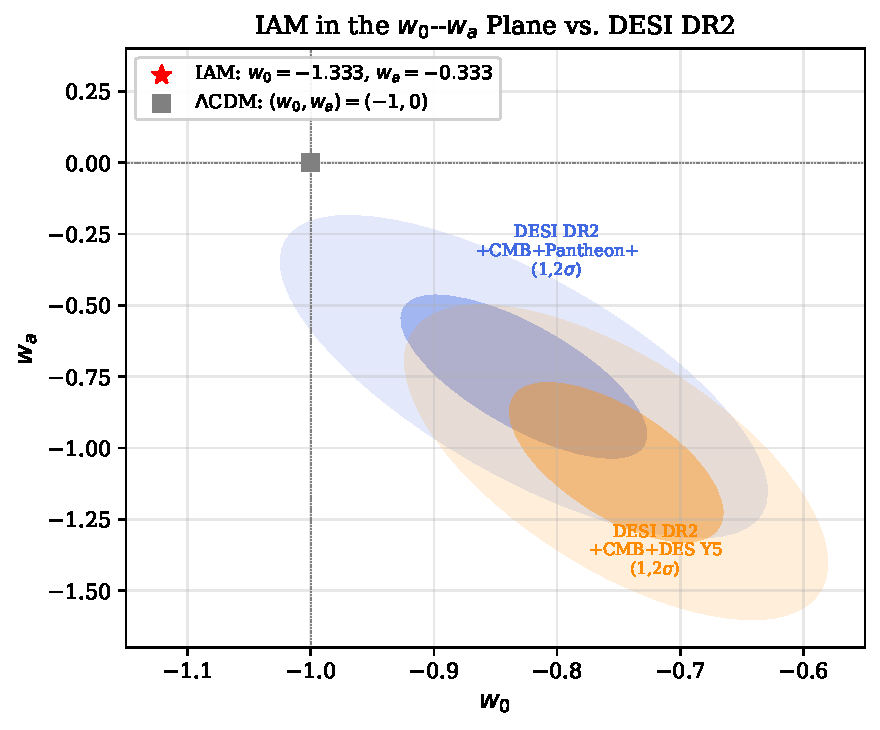
\includegraphics[width=0.72\textwidth]{fig3_desi_w0wa.pdf}
\caption{The \IAM\ prediction (red star) in the $w_0$--$w_a$ plane alongside DESI DR2 1$\sigma$ and 2$\sigma$ contours for DR2+CMB+Pantheon+ (blue) and DR2+CMB+DES~Y5 (orange). The $\Lambda$CDM point $(-1, 0)$ is shown as a gray square. The \IAM\ prediction lies outside the DESI contours but shares the qualitative structure: phantom $w_0$ with a small positive $w_a$. The CPL comparison is imperfect; see Section~\ref{sec:limitations}.}
\label{fig:desi}
\end{figure}

\subsection{Limitations of the CPL Comparison}
\label{sec:limitations}

The $w_0$--$w_a$ parametrization is a Taylor expansion of $w(a)$ around $a = 1$ and is exact only for linear models. \IAM's equation of state $\winfo = -1 - 1/(3a)$ is nonlinear --- it maps to a one-dimensional curve in the infinite-dimensional function space of $w(a)$, and the CPL projection is an approximation that becomes less accurate at $a \ll 1$ or $a \gg 1$.

More importantly, DESI does not measure $w(a)$ directly; it measures BAO distances at discrete redshifts and fits them within the $w_0$--$w_a$ framework assuming that framework is the correct model class. If \IAM\ is the correct model, the DESI BAO distances would need to be fit within the \IAM\ framework --- a different constraint surface in parameter space. The CPL comparison is therefore indicative, not definitive.

The correct comparison is a direct likelihood evaluation of the \IAM\ expansion history against the DESI BAO distance measurements, which is deferred to future work.

\subsection{Falsifiable Predictions}

\IAM\ makes specific, testable predictions for the equation of state as a function of redshift:

\begin{enumerate}
    \item \textbf{$w(z)$ trajectory.} The informational equation of state follows $w(z) = -1 - (1+z)/3$ exactly (substituting $a = 1/(1+z)$). DESI Year~5 will measure $w$ at multiple redshifts with $\sim 1\%$ precision~\citep{DESI2016}. If the data follow the IAM curve rather than a constant $w = -1$ or a CPL-like fit, that is a strong signal. If $w > -1$ is confirmed at any redshift, \IAM\ is disfavored.

    \item \textbf{Asymptotic approach.} At high redshift ($z \gg 1$, $a \ll 1$), the \IAM\ equation of state becomes strongly phantom: $w(z) \approx -1 - (1+z)/3$. This is distinguishable from CPL parametrizations with $w_0 > -1.3$. Future high-$z$ supernova surveys (Nancy Grace Roman Space Telescope) could test this.

    \item \textbf{No Big Rip.} If the equation of state is confirmed to be phantom but trending toward $-1$ over time, consistent with the \IAM\ trajectory, and no Big Rip signature is detected by future surveys, that is consistent with the no-Big-Rip prediction (Section~\ref{sec:heatdeath}).

    \item \textbf{Consistency with growth suppression.} The equation of state prediction and the growth suppression ($\sigma_8 = 0.800$, $\mu < 1$) derive from the same activation function $\Ea$. A survey that simultaneously measures the $w(z)$ trajectory and the growth rate $f\sigma_8(z)$ can test whether both are consistent with the same underlying $\Ea$. This cross-check is unique to \IAM\ and is not reproducible by generic $w_0$--$w_a$ models with separate growth parameters.
\end{enumerate}

% ============================================================
\section{Discussion}
% ============================================================

\subsection{Relation to Existing Dark Energy Models}

\IAM's equation of state $\winfo = -1 - 1/(3a)$ shares the phantom character ($w < -1$) with phantom scalar field models~\citep{Caldwell2002} but differs fundamentally in its mechanism and trajectory. Standard phantom models require a negative kinetic energy term, which violates energy conditions and generically leads to a Big Rip at finite time. \IAM's phantom behavior emerges from the thermodynamics of information encoding, not a negative kinetic term, and is bounded by the saturation of $\Ea$.

The equation of state does not fit cleanly into any existing parametrization class. It is not constant, not CPL, not quintessence. It is derived, with no free parameters, from a specific physical mechanism. This distinguishes it observationally from all fitting functions: the $w(z)$ trajectory is a prediction, not a model.

\subsection{The Inflection Point and the Present Epoch}

The mathematical fact that $E(1)/e = 1/e$ --- that the universe's informational maturity today equals $1/e$, precisely the inflection point of the activation function --- is a consequence of the normalization $E(1) = 1$, which follows from the choice of the Planck epoch as the reference point for the activation function's argument $(1 - 1/a)$.

At this inflection point, the rate of informational maturation $d(E/e)/da$ is maximized. The current epoch is the era of fastest growth in the universe's informational complexity. Structure formation --- the production of irreversible gravitational information through galaxy formation, stellar evolution, and black hole growth --- is occurring at its maximum rate. Observers capable of measuring and interpreting this information have appeared at the moment when the most information is being produced.

Whether this coincidence is physically significant or an artifact of normalization is beyond the scope of this paper. It is noted as a feature of the framework that may merit further investigation.

% ============================================================
\section{Conclusion}
\label{sec:conclusion}
% ============================================================

The Informational Actualization Model derives a specific dark energy equation of state from horizon thermodynamics with zero free parameters: $\winfo = -1 - 1/(3a)$. This equation of state is always mildly phantom, asymptotes toward $-1$ at late times, and excludes the Big Rip scenario through a built-in thermodynamic governor (Equation~\ref{eq:dwda}). The activation function $\Ea$ saturates at $e$, bounding the informational contribution to cosmic expansion and ensuring a final state of informational completion rather than the indefinite dissolution of classical heat death.

The informational maturity framework quantifies where the universe stands in this process: at $a = 1$ today, exactly $1/e \approx 36.8\%$ of the universe's total informational potential has been actualized, at the mathematical inflection point of maximum maturation rate. The maturity milestone table (Table~\ref{tab:maturity}) provides a specific, falsifiable timeline derived from first principles.

The \IAM\ prediction maps to $(w_0, w_a) = (-4/3, -1/3)$ in the CPL parametrization, lying outside current DESI DR2 contours but sharing the qualitative structure of phantom dark energy with a positive $w_a$ (trending toward less phantom). The correct comparison requires fitting the \IAM\ expansion history directly to the BAO distance data, which is deferred to future work.

Three specific tests will determine whether these predictions are correct: DESI Year~5 $f\sigma_8(z)$ measurements at the $\sim 1\%$ level, Rubin-LSST weak lensing growth constraints that simultaneously probe the $\mu < 1$, $\Sigma = 1$ signature and the $w(z)$ trajectory, and Nancy Grace Roman high-$z$ supernova measurements that can distinguish the strongly phantom early-time behavior of $\winfo$ from CPL alternatives. If confirmed, the \IAM\ framework provides a unified physical origin for both the S$_8$ tension and the dark energy evolution currently reported by DESI.

% ============================================================
\section*{Acknowledgments}
% ============================================================

The author thanks the developers of CAMB, MGCAMB, and Cobaya for making cosmological validation accessible to independent researchers. MCMC chains, modified source code, configuration files, and analysis scripts are publicly archived at \url{https://github.com/hmahaffeyges/IAM-Validation}.

% ============================================================
\bibliographystyle{unsrt}
\begin{thebibliography}{99}

\bibitem{Riess1998}
A.~G. Riess et al.,
``Observational Evidence from Supernovae for an Accelerating Universe and a Cosmological Constant,''
\textit{Astron.\ J.}\ \textbf{116}, 1009 (1998).

\bibitem{Perlmutter1999}
S.~Perlmutter et al.,
``Measurements of $\Omega$ and $\Lambda$ from 42 High-Redshift Supernovae,''
\textit{Astrophys.\ J.}\ \textbf{517}, 565 (1999).

\bibitem{PlanckVI2020}
Planck Collaboration,
``Planck 2018 Results. VI. Cosmological Parameters,''
\textit{Astron.\ Astrophys.}\ \textbf{641}, A6 (2020).

\bibitem{DESIDR2_2025}
DESI Collaboration,
``DESI DR2 Results: Baryon Acoustic Oscillations and Dark Energy,''
\textit{arXiv:2503.14738} (2025).

\bibitem{Mahaffey2026_obs}
H.~W. Mahaffey,
``Constraints on Late-Time $f\sigma_8$ Suppression from $\mu < 1$, $\Sigma = 1$: Planck~2018 and Large-Scale Structure,''
submitted to \textit{Universe} (2026).
\url{https://github.com/hmahaffeyges/IAM-Validation}

\bibitem{Mahaffey2026_theory}
H.~W. Mahaffey,
``Dual-Sector Perturbation Cosmology: A Modified CAMB Implementation with $\mu < 1$, $\Sigma = 1$ and the Emergent Hubble Split,''
in preparation (2026).

\bibitem{Mahaffey2026_CAMB}
H.~W. Mahaffey,
``IAM--CAMB Technical Note: Level 2 Validation,''
in preparation (2026).

\bibitem{Jacobson1995}
T.~Jacobson,
``Thermodynamics of Spacetime: The Einstein Equation of State,''
\textit{Phys.\ Rev.\ Lett.}\ \textbf{75}, 1260 (1995).

\bibitem{CaiKim2005}
R.-G. Cai and S.~P. Kim,
``First Law of Thermodynamics and Friedmann Equations of Friedmann--Robertson--Walker Universe,''
\textit{JHEP}\ \textbf{02}, 050 (2005).

\bibitem{Bekenstein1973}
J.~D. Bekenstein,
``Black Holes and Entropy,''
\textit{Phys.\ Rev.\ D}\ \textbf{7}, 2333 (1973).

\bibitem{Hawking1975}
S.~W. Hawking,
``Particle Creation by Black Holes,''
\textit{Commun.\ Math.\ Phys.}\ \textbf{43}, 199 (1975).

\bibitem{GibbonsHawking1977}
G.~W. Gibbons and S.~W. Hawking,
``Cosmological Event Horizons, Thermodynamics, and Particle Creation,''
\textit{Phys.\ Rev.\ D}\ \textbf{15}, 2738 (1977).

\bibitem{CPL2001}
M.~Chevallier and D.~Polarski,
``Accelerating Universes with Scaling Dark Matter,''
\textit{Int.\ J. Mod.\ Phys.\ D}\ \textbf{10}, 213 (2001).

\bibitem{Linder2003}
E.~V. Linder,
``Exploring the Expansion History of the Universe,''
\textit{Phys.\ Rev.\ Lett.}\ \textbf{90}, 091301 (2003).

\bibitem{Caldwell2002}
R.~R. Caldwell,
``A Phantom Menace? Cosmological Consequences of a Dark Energy Component with Super-Negative Equation of State,''
\textit{Phys.\ Lett.\ B}\ \textbf{545}, 23 (2002).

\bibitem{DESI2016}
DESI Collaboration,
``The DESI Experiment: A Whitepaper for Snowmass 2013,''
\textit{arXiv:1308.0847} (2013).

\end{thebibliography}

\end{document}
